\documentclass{article}
\usepackage{graphicx}
\usepackage{amsmath}
\usepackage{amssymb}
\usepackage{authblk}
\usepackage[
backend=biber,
style=numeric,
]{biblatex}
\usepackage{subcaption}
\usepackage{hyperref}
\usepackage{mathptmx}
\usepackage{mathtools}
\usepackage{titling}
\usepackage{fancyhdr}
\usepackage{multirow}
\usepackage{float}
\usepackage{booktabs}
\usepackage[margin=4cm]{geometry}

\addbibresource{refs.bib}

% =============================================
%Import symbols from font cmex without importing the whole package
% =============================================
\DeclareFontFamily{U} {cmex}{}

\DeclareFontShape{U}{cmex}{m}{n}{
  <-6> cmex5
  <6-7> cmex6
  <7-8> cmex7
  <8-9> cmex8
  <9-10> cmex9
  <10-12> cmex10
  <12-> cmex12}{}

\DeclareSymbolFont{Xcmex} {U} {cmex}{m}{n}

%\DeclareMathSymbol{\Xdsum}{\mathop}{Xcmex}{88}% LaTeX can find displaystyle
\DeclareMathSymbol{\Xsum}{\mathop}{Xcmex}{80}

\pretitle{
    \noindent\vrule height 2.5pt width \textwidth
    \huge\bfseries
    \vskip .75em plus .25em minus .25em
    \newline
    \begin{center}
}

\title{\textbf{Advancing Time Series Forecasting: Variance-Aware Loss Functions in Transformers}}
% \title{\textbf{Addressing Bias in Transformer-Based Time Series Forecasting: A Novel Approach to Loss Functions}}

\posttitle{
    \end{center}
    \newline
    \noindent\vrule height 2.5pt width \textwidth
    % \vskip .75em plus .25em minus .25em
}

\preauthor{
    \begin{center}
    \large \lineskip 0.75em
    \vrule height 0.4pt width .5\textwidth\par
    % \begin{tabular}[t]{@{}l@{}}
}
\postauthor{
    % \end{tabular}
    \vskip -.5em
    \par
    \vrule height 0.4pt width .5\textwidth\par
    \end{center}
}

\predate{
    \begin{center}
    \large
}
\postdate{
    \end{center}
}

\author{\textbf{Collin Drake}}
\author{\textbf{Jack Cerullo}}
\affil[1]{Peak to Peak Charter School}

\date{March 1st, 2024}


\begin{document}

\maketitle

\begin{abstract}

When forecasting time series data, transformer models predict sequences lacking in volatility, or bias. We hypothesize that transformer models do so because of their loss functions. More specifically, we posit that the mean component of mean squared error and mean absolute error cause this behavior. We propose two alternative loss functions – Variance-weighted Maximum Squared Error and Variance-weighted Absolute Error – which, crucially, do not incorporate averaging and output variance in the error calculation. We do so to prevent our transformer from converging at a minimum wherein it reduces loss by merely forecasting a time series devoid of volatility, helping time series transformer models continue to train without the risk of underfitting towards the mean. PyTorch implementations of the models used in this project can be found at \href{https://github.com/cldrake01/sibyl}{github.com/cldrake01/sibyl}.

\end{abstract}

\section{Introduction}

In recent years, there has been a surge in efforts to adapt transformers for a wide array of tasks \cite{wen2023transformers}. Landmark models such as the Informer, Autoformer, ETSFormer, and FEDFormer have significantly advanced the field by improving forecast length and accuracy \cite{zhou2021informer, wu2022autoformer, woo2022etsformer, zhou2022fedformer}. Despite notable progress, the application of transformers to time series forecasting remains largely limited, with only a handful of successful implementations such as Google's MetNet-3 \cite{andrychowicz2023deep}. Questions persist regarding their overall effectiveness in time series forecasting \cite{Zeng_Chen_Zhang_Xu_2023}.

Motivated by these concerns, we comprehensively explored and evaluated various transformer-based models. Our investigation revealed a common issue across all models: a tendency towards underfitting, resulting in predominantly unbiased, ``linear" predictions regardless of the transformer architecture employed. Fig.(1) shows this underfitting.

\begin{figure}[!tbp]
  \centering
  \begin{minipage}[b]{0.49\textwidth}
    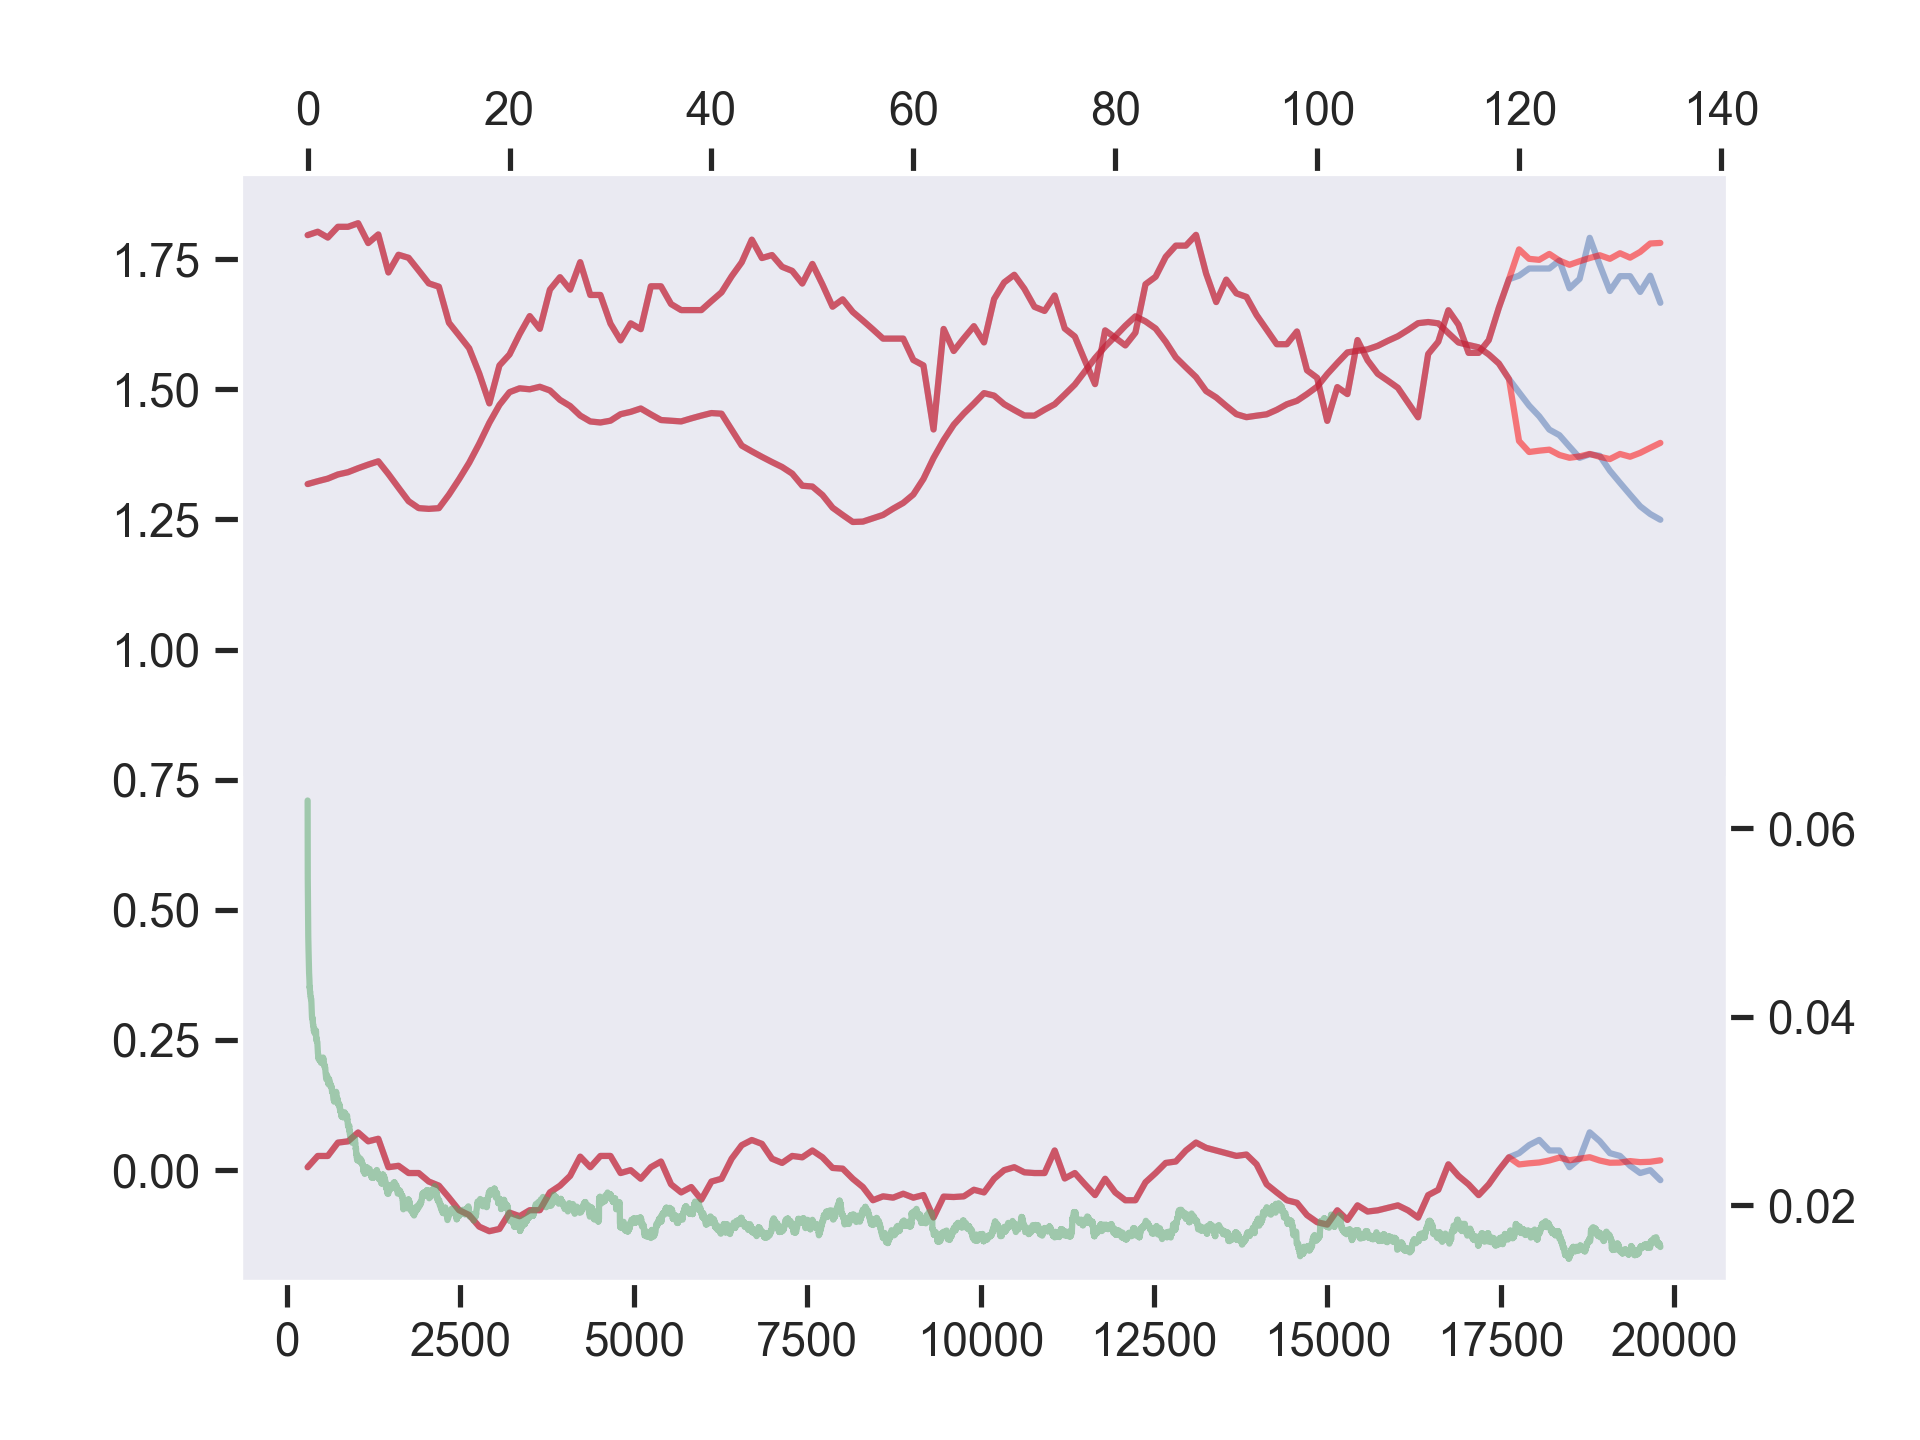
\includegraphics[width=\textwidth]{paper/imgs/mse.png}
    \subcaption{MSE}
  \end{minipage}
  \hfill
  \begin{minipage}[b]{0.49\textwidth}
    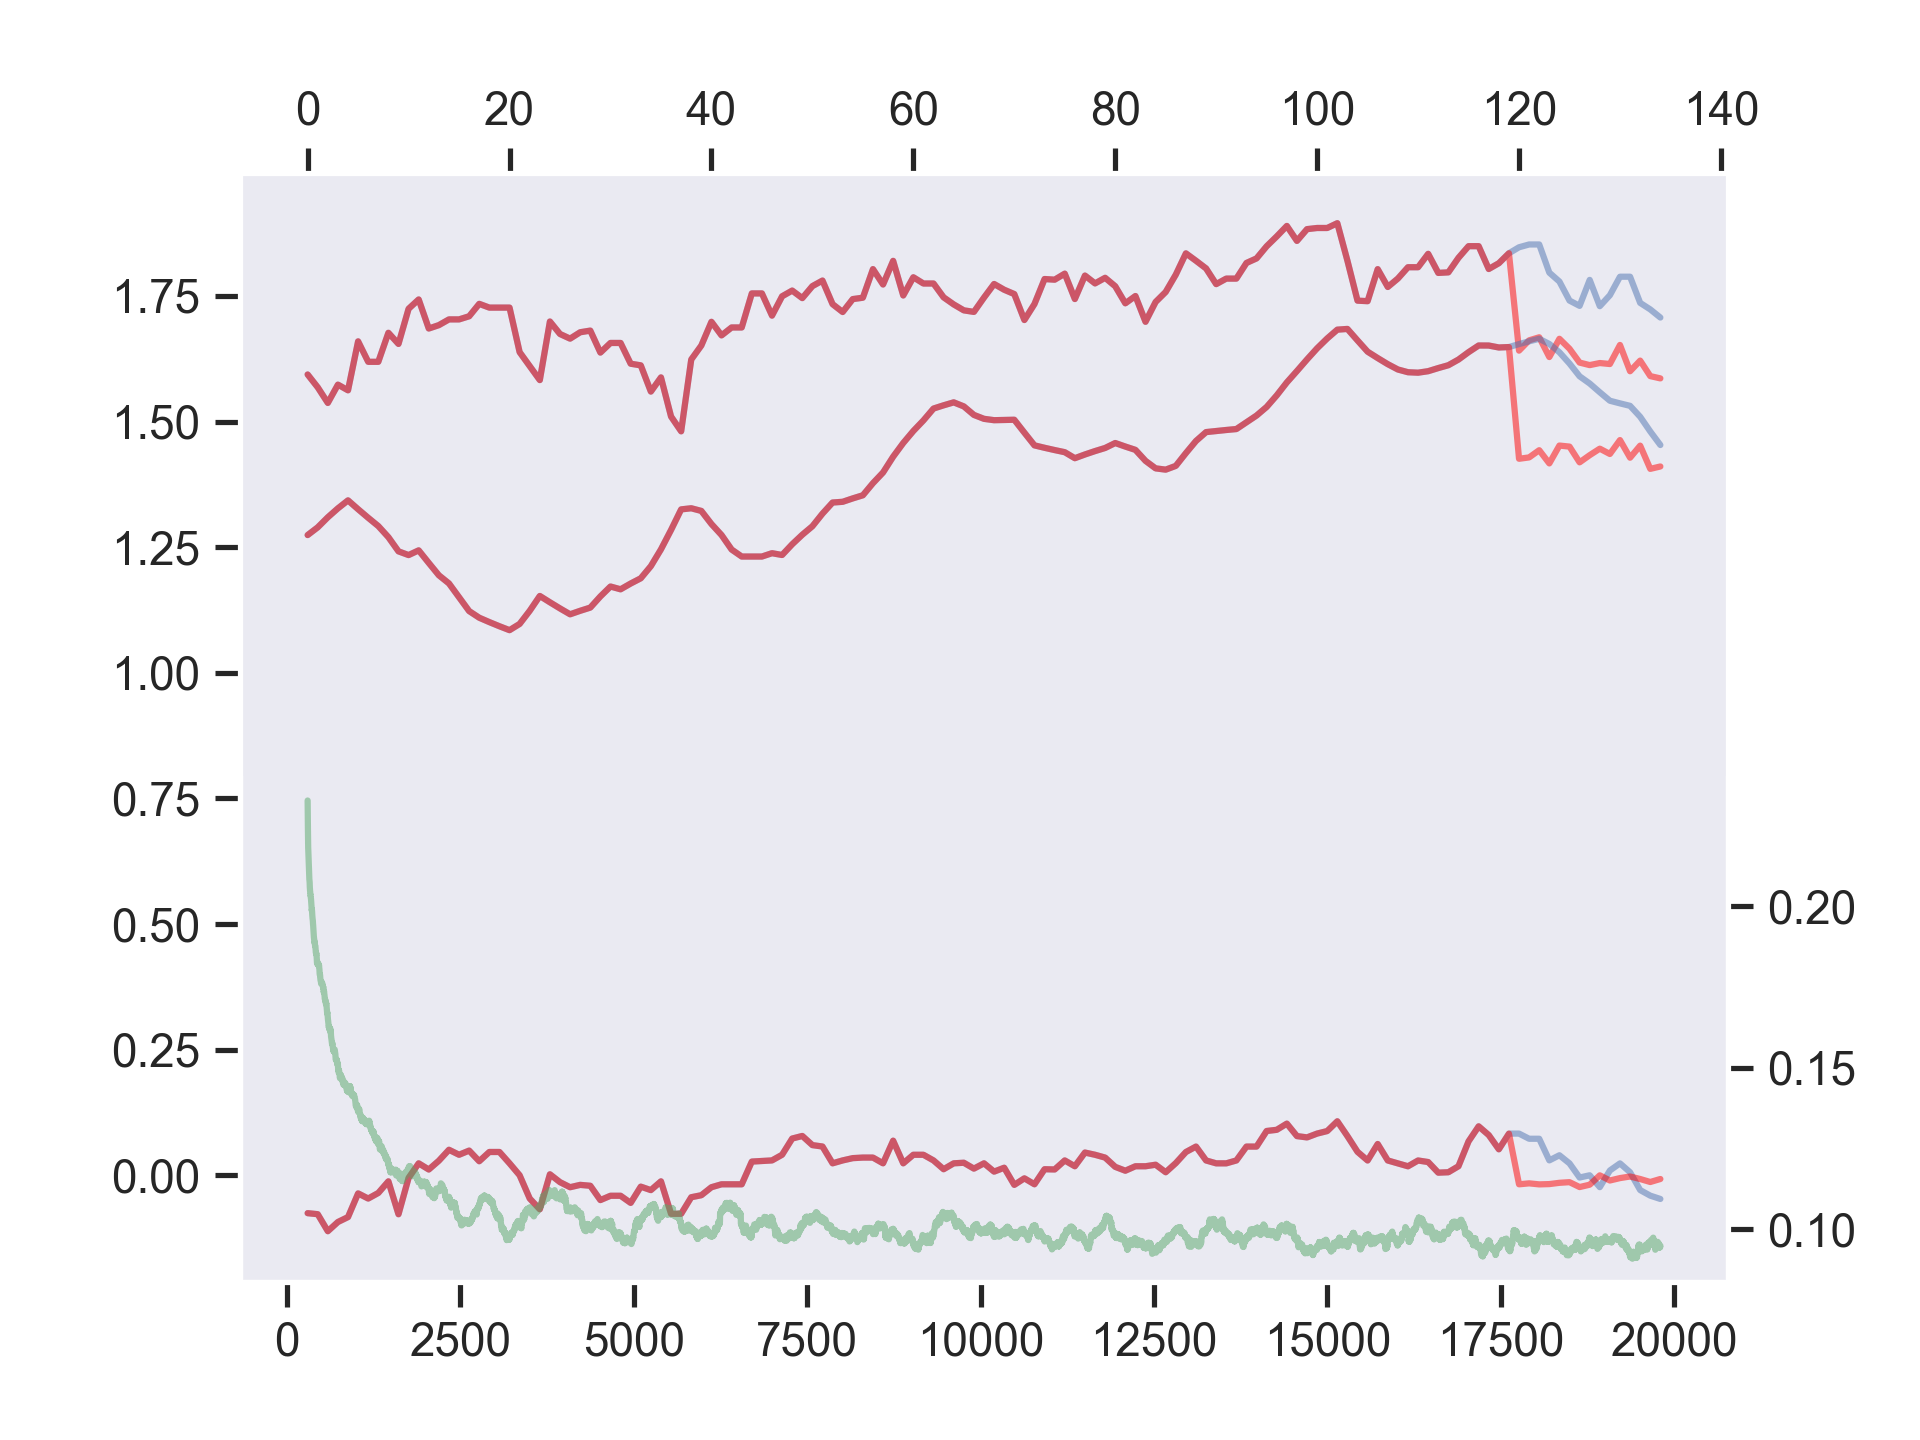
\includegraphics[width=\textwidth]{paper/imgs/mae.png}
    \subcaption{MAE}
  \end{minipage}
  \caption{The model's predictions (red) exhibit insufficient volatility compared to the actual values (blue). The green subplots display MSE and MAE on the right and left respectively. In other words, the model is severely underfitted.}
  \label{fig:MSE & MAE}
\end{figure}

Such behavior is detrimental to transformers in any sort of application wherein a certain volatility is expected of the forecasted sequence. Admittedly, the prevalence of this underfitting across models perplexed us for some time. Eventually, we concluded that the existence of a minimum that punished deviation from the actual sequence's mean was, naturally, owed to the mean component of mean squared error and mean absolute error.

Armed with this information, we then took a step back to examine Mean Squared Error (MSE) and Mean Absolute Error (MAE). We noticed two things: firstly, metrics that optimize for a mean lead to underfitting; secondly, these metrics consider each time step to be equally important when in reality, the final value of a time series is often most crucial.

Our proposed loss functions seek to mitigate the observed lack of bias by optimizing for the variance, or ``shape", of our time series instead. Hereafter, we'll explore various alternatives to averaging the residuals, and we'll also explore weighting and other heuristics.

\section{Related Work}

\subsection{Loss Functions}

As it stands, the prevailing issue amongst MSE and other such \( L_p \) norm variants is such that they're insensitive to the shape of data. By nature of mean being their key component, they will, of course, aim to reduce the mean error. This results in the characteristically invariant, or flat in ``shape", when MSE or MAE are applied to time series forecasting. In 2024, Lee et al. attempted to mitigate this issue with TILDE-Q, but, whilst innovative, this method achieves results only marginally better than their benchmark \cite{lee2024tildeq}.

Computer vision has also seen some innovative loss functions which optimize for depth estimation and generative image synthesis \cite{Barron_2019_CVPR}.

\subsection{Transformer Architectures}

Researchers and practitioners have long been interested in autoregressive models for their ability to forecast a wide array of trends, the applications of which include weather forecasting, demand forecasting, and quantitative analysis \cite{doi:10.1177/1847979018808673, andrychowicz2023deep, HO1998213, 10146913}. Autoregressive models, including ARIMA, RNNs, LSTMs, as well as N-BEATS \cite{DBLP:journals/corr/abs-1905-10437} and N-HITS \cite{challu2022nhits} more recently, have been extensively used in forecasting tasks but often struggle with capturing long-term dependencies, especially in seemingly stochastic time series data \cite{9005997, LINDEMANN2021650, KAREVAN20201, 8614252, CAO2019127, SAGHEER2019203}. Transformers, however, are known for their wildly successful application to Natural Language Processing (NLP) tasks, wherein they are required to attend to the relationships of many interdependent tokens. It was for their ability to capture long-term dependencies and complex relationships that researchers began applying transformers to time series forecasting tasks. Consequently, researchers have seen many new transformer architectures in recent years, with many of them having been conceived with time series forecasting in  mind \cite{zhou2021informer, wu2022autoformer, liu2023ring, brandon2023striped}. While transformers have come a long way, each architecture that we tested exhibited significant underfitting when tasked with forecasting stochastic, financial data.

\section{Methodology}

\subsection{Existing Loss Functions}

It's worth noting that actual values,  \( \mathbf{y} \), and the predicted values, \( \mathbf{ \hat{y} }\), are always assumed to be identical in their lengths, e.g.,  \( n = \text{dim} \left( \mathbf{y} \right) = \text{dim} \left( \mathbf{\hat{y}} \right) \). For regression, the most widely used loss functions are

\begin{align*}
    \text{MSE}
    &= \frac{1}{n} \Xsum^{n}_{i=1} \left( \mathbf{y}_i - \mathbf{\hat{y}}_i \right)^2,
    \\[30pt]
    \text{MAE}
    &= \frac{1}{n} \Xsum^{n}_{i=1} \left| \mathbf{y}_i - \mathbf{\hat{y}}_i \right|.
\end{align*}

\subsection{Maximum Error}

Maximum Error functions are practically the same function as Mean Error Functions (MAE, MSE), with the only difference being that they take the maximum difference within the residuals as opposed to a mean difference. We use this function to create more of a ``moving target" for our model to target, as opposed to solely minimizing a mean of the residuals.

\begin{align*}
    \text{MaxSE}
    &= \text{max} \left( \left( \mathbf{y} - \mathbf{\hat{y}} \right) ^2 \right) \\
    &= \underset{\forall i \in n}{\text{max}} \left( \; \left( \mathbf{y}_i - \mathbf{\hat{y}}_i \right)^2 \right),
    \\[30pt]
    \text{MaxAE}
    &= \text{max} \left( \left| \mathbf{y} - \mathbf{\hat{y}} \right| \right) \\
    &= \underset{\forall i \in n}{\text{max}} \left( \left| \mathbf{y}_i - \mathbf{\hat{y}}_i \right| \right).
\end{align*}

\subsection{Variance-weighted Maximum Error}

We incorporate the absolute difference in variances to ensure that \( \mathbf{\hat{y}} \) has a similar variance to that of \( \mathbf{y} \). We raise \( e \) to the power of our maximum differences for two reasons: firstly, to raise our differences above 1; and secondly, to penalize larger differences in variance. Differences in variance can be thought of as differences in ``shape".

\begin{align*}
    \text{VMaxSE}
    &= \text{exp} \left( \left( \text{var}(\mathbf{y}) - \text{var}(\hat{\mathbf{y}}) \right)^2 \right)
    \cdot \text{max} \left( \left( \mathbf{y} - \mathbf{\hat{y}} \right)^2 \right) \\
    &= \text{exp} \left( \left( \text{var} \left( \mathbf{y} \right) - \text{var} \left( \hat{\mathbf{y}} \right) \right)^2 \right)
    \cdot \underset{\forall i \in n}{\text{max}} \left( \left( \mathbf{y}_i - \mathbf{\hat{y}}_i \right)^2 \right) ,
    \\[30pt]
    \text{VMaxAE}
    &= \text{exp} \left( \left| \text{var}(\mathbf{y}) - \text{var}(\mathbf{\hat{y}}) \right| \right)
    \cdot \text{max}  \left( \left| \mathbf{y} - \mathbf{\hat{y}} \right| \right) \\
    &= \text{exp} \left( \left| \text{var}(\mathbf{y}) - \text{var} \left( \hat{\mathbf{y}} \right) \right| \right)
    \cdot \underset{\forall i \in n}{\text{max}} \left( \left| \mathbf{y}_i - \mathbf{\hat{y}}_i \right| \right) .
\end{align*}

\section{Results}

After benchmarking, we've found that VMaxSE and VMaxAE increase bias while reducing variance accross all datasets.

\begin{table}[htbp]
  \centering
  \caption{Bias and Variance for Multiple Datasets}
  \label{tab:dataset_metrics}
  \begin{tabular}{lccccccc}
    \toprule
    & \multicolumn{2}{c}{Alpaca} & \multicolumn{2}{c}{ETT} & \multicolumn{2}{c}{ELD} \\
    \cmidrule(lr){2-7}
    & Bias & Variance & Bias & Variance & Bias & Variance \\
    \midrule
    VMaxSE  & 0.09222 & 0.52092  & 0.50260 & 0.05046  & 0.48630 & 0.01289 \\
    MSE     & 0.08829 & 0.53864  & 0.28703 & 0.07763  & 0.34997 & 0.09874 \\
    VMaxAE  & 0.09223 & 0.52484  & 0.50944 & 0.04321  & 0.39521 & 0.06571 \\
    MAE     & 0.08830 & 0.54095  & 0.25954 & 0.08988  & 0.30059 & 0.22571 \\
    \bottomrule
  \end{tabular}
\end{table}

\begin{figure}[!tpb]
  \centering
  \begin{minipage}[b]{0.49\textwidth}
    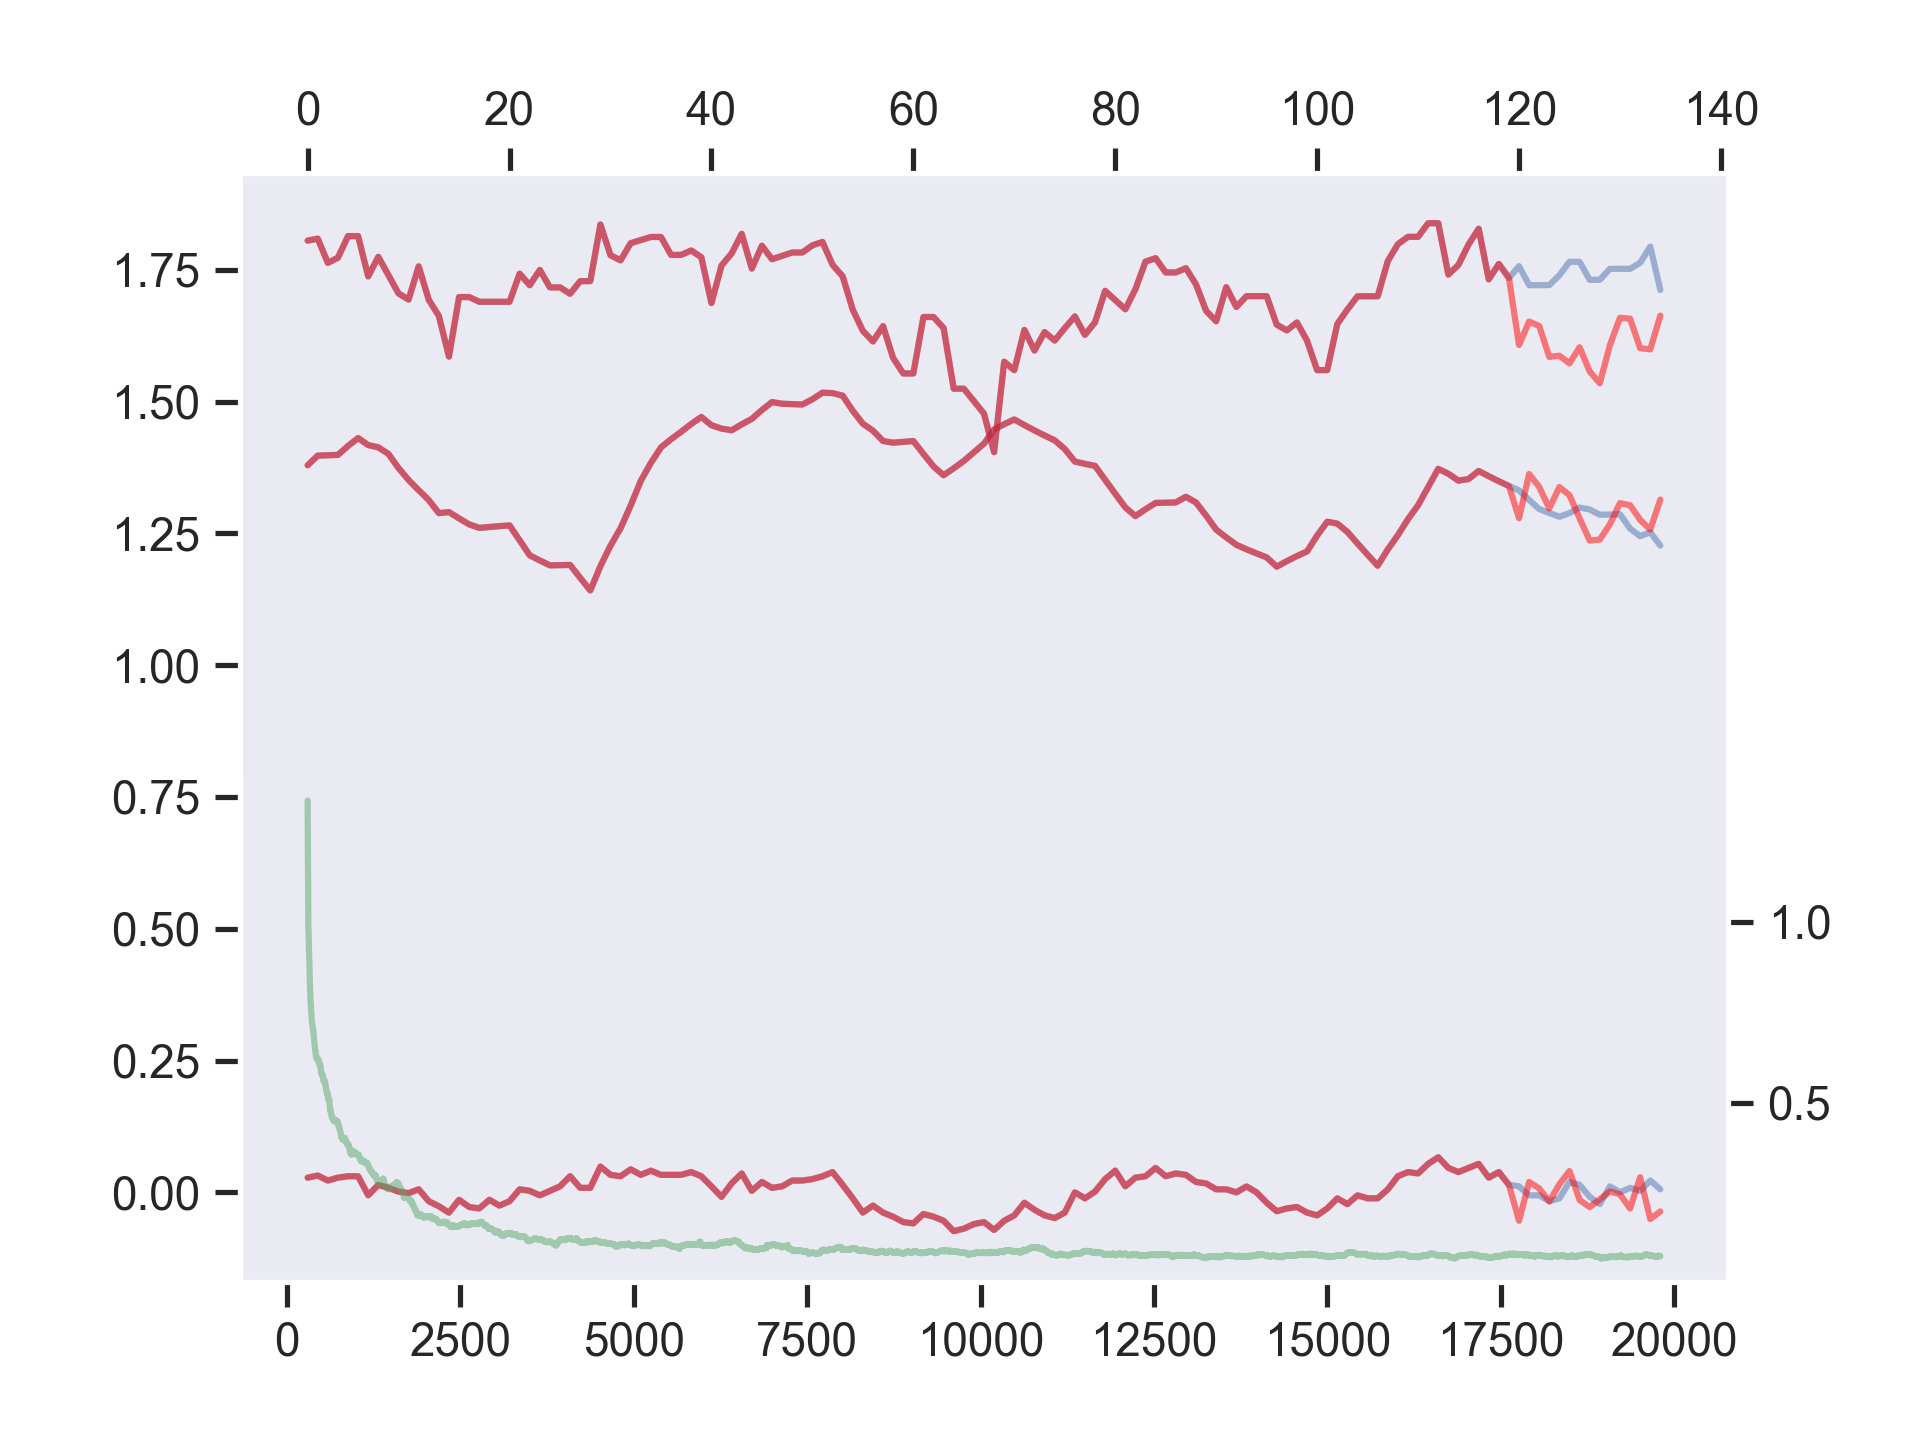
\includegraphics[width=\textwidth]{paper/imgs/vmaxse.png}
    \subcaption{VMaxSE}
  \end{minipage}
  \hfill
  \begin{minipage}[b]{0.49\textwidth}
    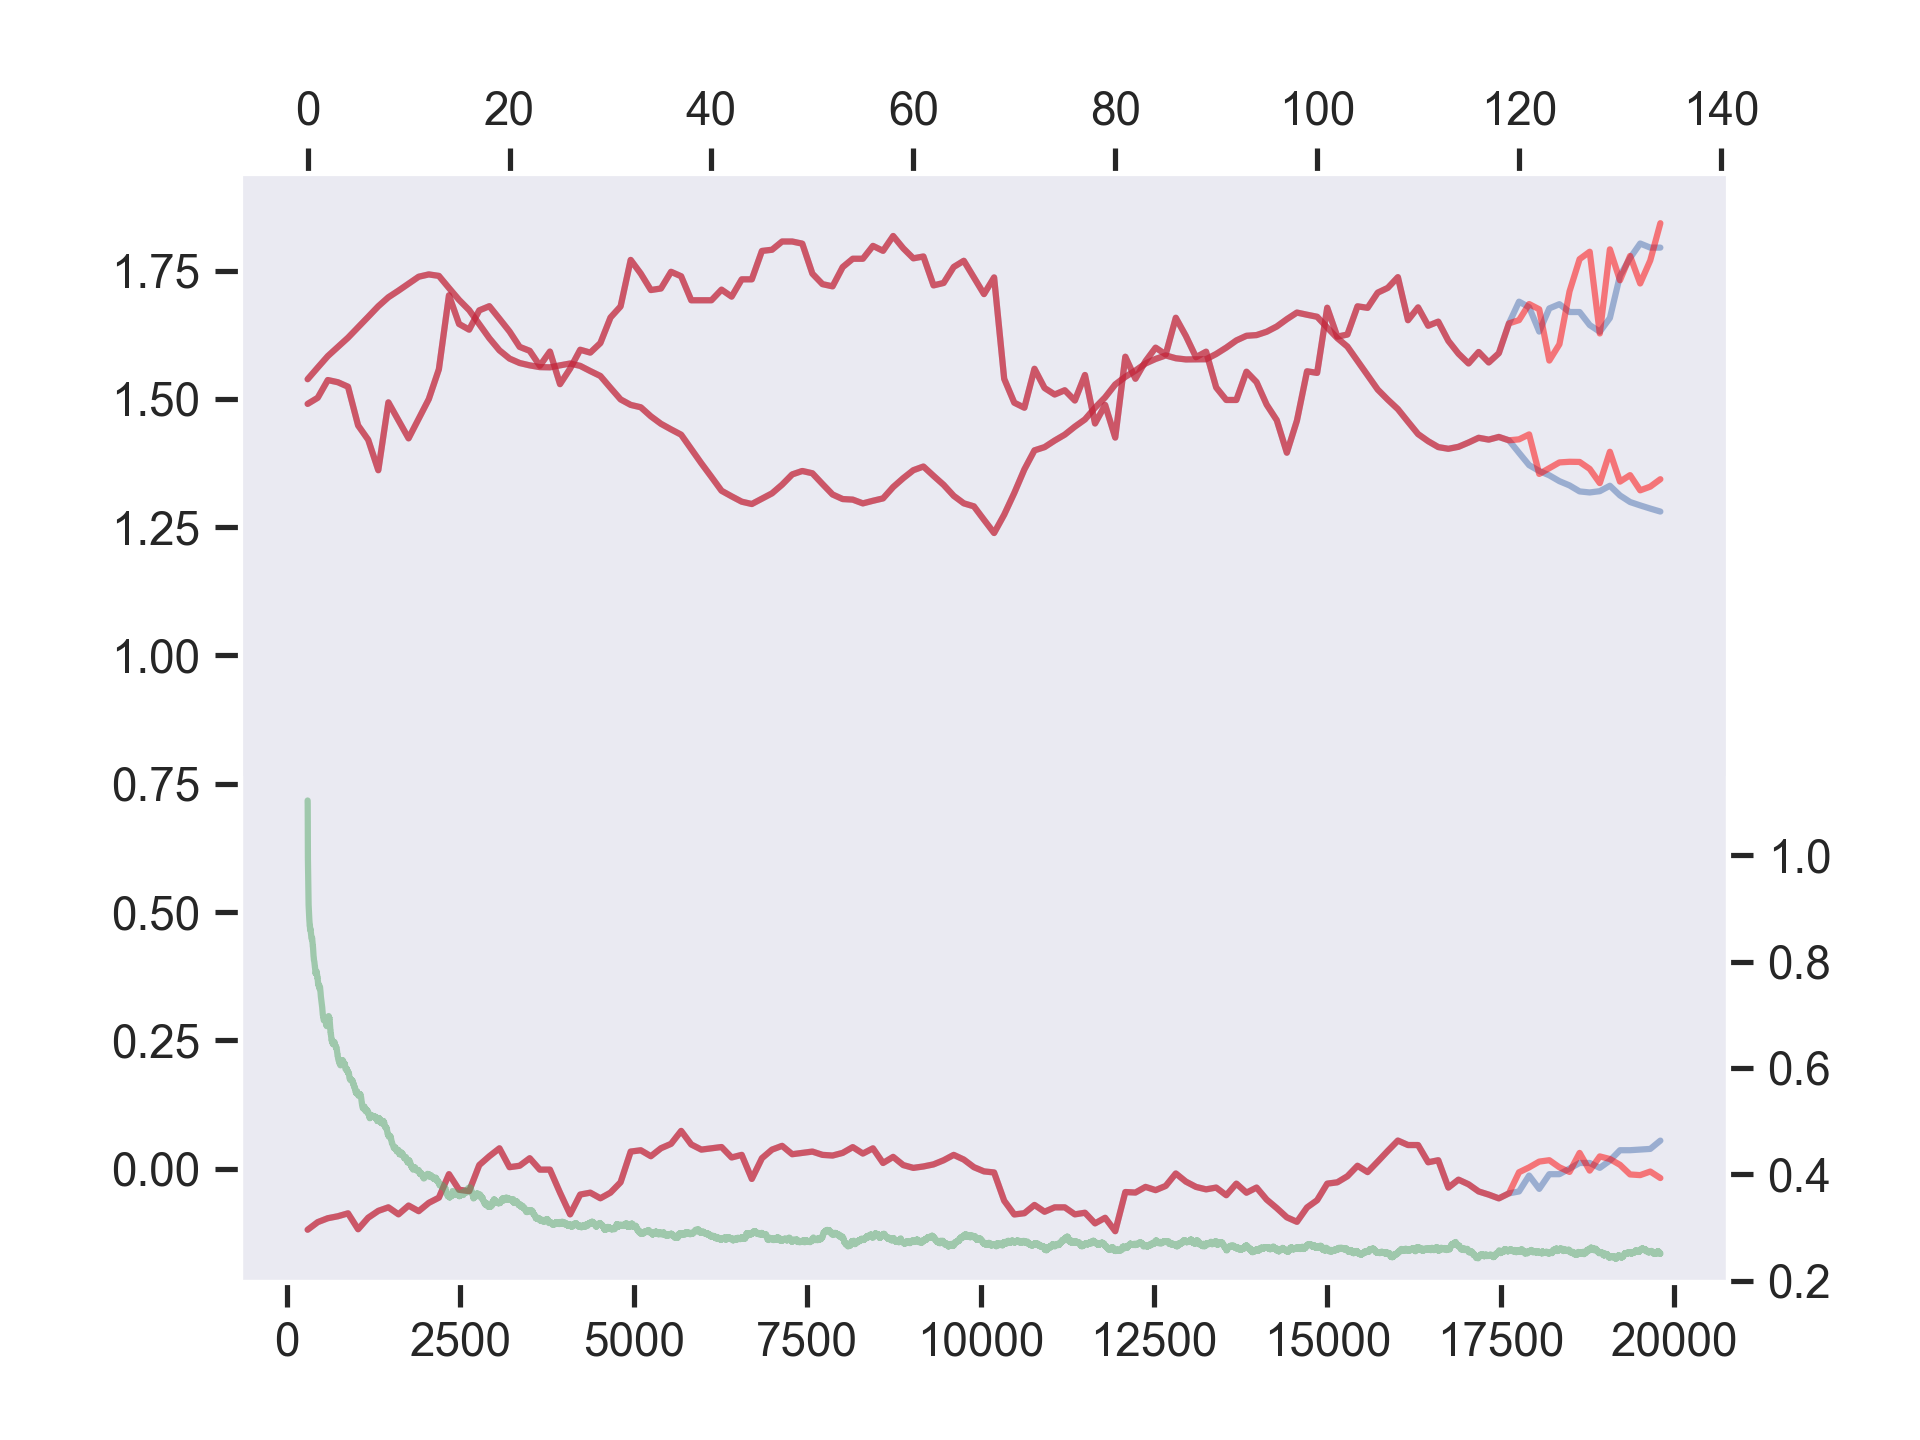
\includegraphics[width=\textwidth]{paper/imgs/vmaxae.png}
    \subcaption{VMaxAE}
  \end{minipage}
  \caption{The model's predictions (red) exhibit similar volatility compared to the actual values (blue). The green subplots distplay MSE and MAE on the right and left respectively.}
  \label{fig:VMaxSE & VMaxAE}
\end{figure}

\section{Conclusion}

In summary, our study addressed the issue of underfitting and unbiased predictions in transformer-based time series forecasting models, attributing it to the mean component in traditional loss functions like MSE and MAE. To counter this lack of bias, we introduced two variance-weighted loss functions, VMaxSE and VMaxAE, which prioritize capturing the shape of the time series over averaging. Our experiments demonstrated the effectiveness of these loss functions in improving prediction accuracy, volatility, and bias. This underscores the necessity of rethinking loss functions in time series forecasting, especially in transformer models, for more accurate predictions. We anticipate further exploration of innovative loss functions and architectural improvements to address underfitting by considering the temporal characteristics of data.

The datasets used can be found at these references:

\href{https://github.com/zhouhaoyi/ETDataset}{github.com/zhouhaoyi/ETDataset},

\href{https://www.ncei.noaa.gov/data/local-climatological-data}{www.ncei.noaa.gov/data/local-climatological-data},

\href{https://archive.ics.uci.edu/dataset/321/electricityloaddiagrams20112014}{archive.ics.uci.edu/dataset/321/electricityloaddiagrams20112014}

\section{Acknowledgements}

We would like to thank our teachers who helped us with this project, specifically Mr. Robert Hettmansperger, Mr. Jake Lehr, and Mx. Seonjoon-young.

\printbibliography

\end{document}
